\section{Importing MIDI Files}\label{importMIDI}

blue is able to import MIDI files and set up a blue project file from
the note information in the MIDI file, using the settings given by the
user. To import a MIDI file, choose the "Import MIDI File" option from
the File menu. Next, using the file dialog to locate the MIDI file to
import. After selecting the desired file, blue will show the following
MIDI Import Settings dialog for you to configure how you would like to
import the MIDI note information. (Note: blue will only show information
for tracks where note data was found.)

MIDI Import Settings

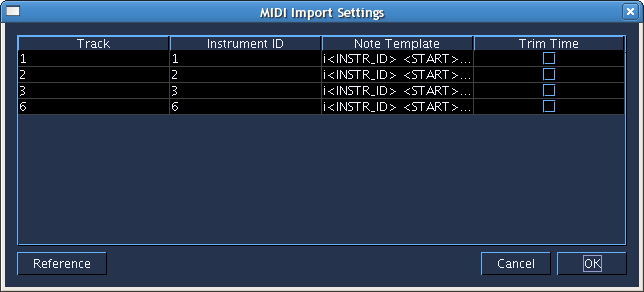
\includegraphics{images/midiImportSettings.png}

The table column information is as follows:

\begin{description}
\item[Track]
The original MIDI track number to which this setting is to be applied
to. This column is not editable is for reference purpose only.
\item[Instrument ID]
The Csound instrument ID to use for this track. This will replace the
\textless{}INSTR\_ID\textgreater{} key within the note template. This
value is treated as a string to allow users to assign the track
information to Csound named instruments. If one is doing so, one must
quote the name, i.e. use "trumpet" instead of trumpet (without quotes),
otherwise the output will not be legal Csound SCO. Default value is the
number of the MIDI track.
\item[Note Template]
Template note text to use for generating Csound SCO from the MIDI data.
The default note template is "i\textless{}INSTR\_ID\textgreater{}
\textless{}START\textgreater{} \textless{}DUR\textgreater{}
\textless{}KEY\textgreater{} \textless{}VELOCITY\textgreater{}". By
having note templates, the user can massage the note information to work
with any number of pfields that their instruments require.

The following values are allowed in the note template:

\begin{longtable}[]{@{}ll@{}}
\caption{Key Values}\tabularnewline
\toprule
Shortcuts & Description\tabularnewline
\midrule
\endfirsthead
\toprule
Shortcuts & Description\tabularnewline
\midrule
\endhead
\textless{}INSTR\_ID\textgreater{} & The instrument ID assigned in the
track settings.\tabularnewline
\textless{}START\textgreater{} & Start Time of Note\tabularnewline
\textless{}DUR\textgreater{} & Duration of Note\tabularnewline
\textless{}KEY\textgreater{} & MIDI key number\tabularnewline
\textless{}KEY\_PCH\textgreater{} & MIDI key number as Csound
PCH\tabularnewline
\textless{}KEY\_OCT\textgreater{} & MIDI key number as Csound
OCT\tabularnewline
\textless{}KEY\_CPS\textgreater{} & MIDI key number as
CPS\tabularnewline
\textless{}VELOCITY\textgreater{} & MIDI velocity number\tabularnewline
\textless{}VELOCITY\_AMP\textgreater{} & MIDI velocity number as
amplitude\tabularnewline
\bottomrule
\end{longtable}

The button labelled "Reference" on the dialog will pop open the above
information for quick reference of the allowable replacement keys for
note templates.
\item[Trim Time]
This option will shift the generated SoundObject to the time of the
first note and then take the generated notes for the track and shift
them all so that the first note starts at time 0 so that there is no
empty time at the beginning of the track's note information.
\end{description}

After finishing configuring settings for the imported MIDI data, blue
will generate the notes with one SoundLayer per MIDI track, and on each
SoundLayer it will contain one GenericScore SoundObject containing the
converted MIDI score.

\begin{quote}
\textbf{Note}

The current implementation does not handle cases where there are
overlapping notes of the same MIDI note number within the same track and
results are unpredictable. Also, only MIDI files where time is PPQ is
supported at the moment (non-SMPTE). Users wanting support for either of
these cases or have other ideas they would like implemented are
requested to make feature requests on the blue mailing list or to use
the help menu "Request a Feature" option.
\end{quote}
